\section{UnsolvableQA Construction}
\label{sec:dataset}

Most existing benchmarks primarily focus on solvable tasks, which often leads to hallucinations during feasibility evaluations. To better understand this issue,  we present UnsolvableQA using a dual-track methodology tailored to domain-specific verification (Figure~\ref{fig:pipeline}).

\subsection{Mathematical Data Collection}
\label{sec:math_gen}

Programmatic verification is often infeasible for advanced math tasks. We therefore use \textbf{Reverse Construction} for the entire mathematical unsolvable-data pipeline (Figure~\ref{fig:pipeline}a): starting from solvable seed problems and verified solution paths, we reverse-engineer input-side flaws that make the final answer undefined. The pipeline has two stages:

\vspace{0.3em}
\noindent\textbf{Data Generate Process.}
First, we filter seed problems, retaining only those where a strong LLMs (DeepSeek-Reasoner) successfully generates a correct result. Next, the same model plans and injects controlled constraint conflicts into the problem statement, such as mutually incompatible conditions or externally added constraints that make the original solution path invalid. Guided by the structural plan, these conflicts are precisely targeted within the problem statement while preserving the surface form of a plausible reasoning problem.

\vspace{0.3em}
\noindent\textbf{Validation Process.}
We further implement a multi-tier verification protocol. First, the generated problem is presented to DeepSeek-R1 for autonomous contradiction detection. If the model fails to identify the flaw independently, we provide it with the predefined contradiction plan to reassess solvability.
To ensure logical rigor, we introduce a \textbf{Consensus-Based Cross-Verification} stage where Gemini 3 Pro evaluates the generated instance against the intended contradiction. If Gemini identifies loopholes, the two models engage in an iterative debate. An instance is retained only if both models reach a unanimous consensus on its unsolvability. Ultimately, three STEM Master's students manually audited the entire test set to guarantee data quality and logical consistency (detailed in Appendix~\ref{subsec:reverse_pipeline}).




\subsection{Puzzle Data Collection}
\label{sec:logic_gen}

We developed automated generators for four representative domains (Figure~\ref{fig:pipeline} (b)), employing deterministic solvers to guarantee strict unsolvability across all instances.

\paragraph{Game24.} 
We enumerate all binary expression trees using exact rational arithmetic (Python Fraction) to avoid floating-point errors. Unsolvable instances are isolated via \textit{rejection sampling} of number sets mathematically proven to lack solutions.

\paragraph{Hamiltonian Cycle/Path.}
Graph traversability is framed as a SAT problem and verified via pysat (MiniSat). We engineer unsolvable instances by injecting structural impossibilities, such as severing critical edges or creating bottlenecks.

\begin{figure*}[t]
    \centering
    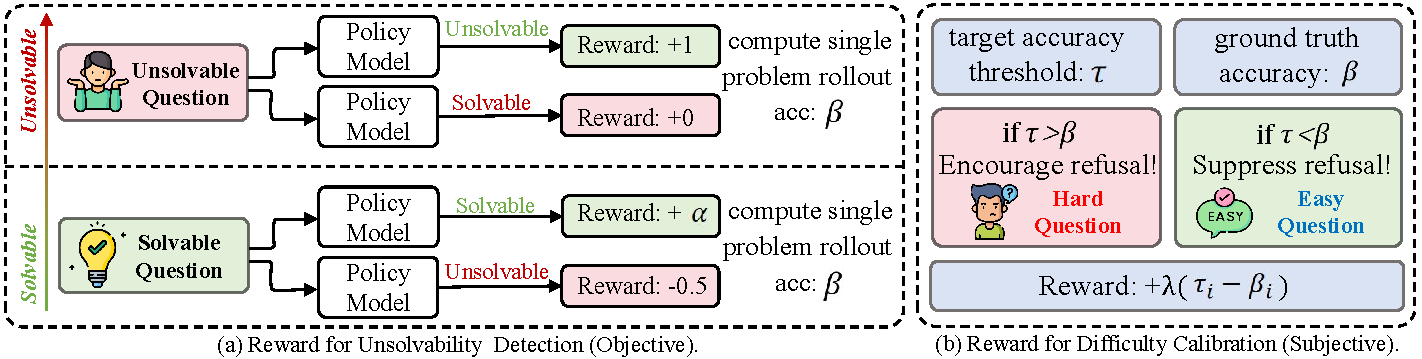
\includegraphics[width=\linewidth]{figures/reward_.pdf}
    \caption{UnsolvableRL reward design. The framework decouples three behaviors: reasoning accuracy on solvable instances, unsolvability detection for input-side defects, and capability calibration for solvable but currently hard instances. Panel (a) visualizes the objective solvability reward, including correctness reward on solvable queries, unsolvability reward on flawed queries, and a false unsolvability penalty for labeling solvable queries as unsolvable. Panel (b) visualizes capability calibration, which regulates \texttt{<beyond\_capacity>} refusal by comparing the target threshold \(\tau\) with the ground-truth-verified rollout accuracy \(\beta\): refusal is encouraged when \(\tau>\beta\) and discouraged when \(\tau<\beta\).}
    % {\textcolor{red}{Revise the image.}}}
    \label{fig:reward_design}
\end{figure*}

\paragraph{Hitori.}
We model Hitori as a constraint satisfaction problem using python-constraint. Unsolvable variants are generated by injecting conflicting constraints, such as forcing duplicate numbers that violate fundamental adjacency rules.

\paragraph{Maze Navigation.}
Base mazes are generated via randomized DFS. To ensure unsolvability, we obstruct a \textit{critical junction} shared by all valid paths and verify the resulting impossibility via BFS.

\begin{table}[t]
    \centering
    
    
    \resizebox{\linewidth}{!}{%
    \begin{tabular}{llccc}
        \toprule
        \textbf{Split} & \textbf{Domain} & \textbf{Solvable} & \textbf{Unsolvable} & \textbf{Total} \\
        \midrule
        Train & Game24 & 50 & 50 & 100 \\
        Train & Hamiltonian Cycle & 48 & 48 & 96 \\
        Train & Hamiltonian Path & 50 & 50 & 100 \\
        Train & Hitori & 50 & 50 & 100 \\
        Train & Maze & 100 & 59 & 159 \\
        Train & AIME (1983--2023) & 50 & 32 & 82 \\
        \midrule
        Test & Game24 & 50 & 50 & 100 \\
        Test & Hamiltonian Cycle & 48 & 50 & 98 \\
        Test & Hamiltonian Path & 50 & 50 & 100 \\
        Test & Hitori & 50 & 50 & 100 \\
        Test & Maze(Easy) & 100 & 94 & 194 \\
        Test & Maze(Hard) & 100 & 100 & 200 \\
        Test & AIME (2024--2025) & 60 & 47 & 107 \\
        \midrule
        Train  & Total & 348 & 289 & 637 \\
        Test  & Total & 458 & 441 & 899 \\
        \bottomrule
    \end{tabular}}
    \caption{Unified vertical statistics for \textbf{UnsolvableQA} train/test partitions. Train Maze has no difficulty split; AIME year ranges differ.}
    \vspace{-5pt}
    \label{tab:dataset_stats}
\end{table}
\subsection{Dataset Statistics and Quality Control}
\textbf{UnsolvableQA} is domain-balanced (Table~\ref{tab:dataset_stats}), comprising 899 test instances (458 solvable, 441 unsolvable) and 637 training instances (348 solvable, 289 unsolvable). Training prompts utilize templated formats with aggregated difficulties, whereas test prompts are diverse and preserve fine-grained splits, including disjoint AIME years\footnote{AIME year ranges: train 1983--2023; test 2024--2025.}. For rigorous quality control, logic puzzles are verified via rule-based solvers, while math problems undergo multi-pass LLM validation and manual review. Detailed construction of the fine-grained diagnostic dataset, categorized by Missing Information (MI) and Constraint Conflict (CC), along with two additional out-of-distribution test sets, are provided in Appendix~\ref{sec:appendix_data_detail} and~\ref{sec:appendix_ood}, respectively.
